\chapter{Exploring Uncertainty Quantification} \label{txt:uncertainty-chapter}

The prudent Icarus-RSM architecture introduced in \Cref{txt:icarus-rsm} consists of an out-of-distribution detector, a prediction model, and an uncertainty quantifier. While \Cref{txt:ood-detection-chapter} and \Cref{txt:prediction-chapter} have already explored the first two components, the following chapter analyses the capabilities of different uncertainty quantification methods. First, \Cref{txt:uncertainty-methods} introduces the methods we use to evaluate and visualise the performance of the uncertainty quantifiers. The following sections analyse several methods, such as directly predicting the uncertainty level $\sigma$ (\Cref{txt:uncertainty-predict-sigma}), estimating the prediction model's error (\Cref{txt:uncertainty-predict-error}), learning the shape of prediction intervals (\Cref{txt:uncertainty-predict-range}), and ensemble methods (\Cref{txt:uncertainty-ensemble-methods}). Finally, \Cref{txt:uncertainty-conclusions} offers brief conclusions and recommendations for choosing an uncertainty quantifier for the Icarus RSM.

\section{Methods for Evaluating Uncertainty Quantifiers} \label{txt:uncertainty-methods}

In the three-module Icarus-RSM architecture, the responsibilities of OOD detection and uncertainty quantification are clearly separated. In particular, the uncertainty quantifier is only responsible for estimating the prediction uncertainty of the prediction model under the assumption that a prediction \textit{can} be made. Specifically, the uncertainty estimate is conditioned on the OOD detector's confidence that an input is in-distribution. Therefore, this chapter only evaluates the uncertainty quantifiers on in-distribution and most-likely-ID inputs. Each quantifier is paired with a prediction model, which is first trained on the combined training data from all six trajectories (see \Cref{txt:six-trajectories}). Crucially, the quality of the predictions themselves is not the focus of this chapter. Some methods like Gaussian processes or Random Forest ensembles combine predictor and uncertainty quantifier in one method and thus only need this first step of training. However, if they are separate methods, the uncertainty quantifier is now trained on the prediction errors of the predictor for a held-out subset of the training data. Finally, the quantifiers are evaluated on the combined testing data from all six trajectories and their $-4\text{h}$, $-2\text{h}$, $-1\text{h}$, $+1\text{h}$, $+2\text{h}$, and $+4\text{h}$ neighbours. This enlarged test dataset ensures that a larger variety of prediction errors can be analysed and that the inputs we evaluate the quantifier on share many common features due to temporal proximity and are thus likely still in-distribution.

\newpar In this chapter, the performance of each uncertainty quantifier is evaluated using a three-panel figure per quantifier. For each figure, the panel on the left names the method and plots the prediction model's prediction error $y - \hat{y}$ against the uncertainty quantifier's uncertainty estimate $\hat{\sigma}$ in a two-dimensional histogram. The CET-L8 colour scheme \cite{color-cet-2015, color-cet-2023} is used to encode the frequency of error-uncertainty pairs in each bin. Empty bins are coloured white, and non-empty bins range from blue for lower frequencies over red to yellow for higher frequencies. Since a well-trained model generally predicts fewer larger errors, the histogram would naturally show higher frequencies close to zero prediction error. We normalise the frequencies in each column of the 2D histogram, i.e. amongst different uncertainties for similar prediction errors, such that the data distribution bias towards lower errors does not distort the colour-coding of the bin frequencies. An ideal uncertainty quantifier would generally predict higher uncertainty for higher absolute prediction errors and would not differentiate between positive and negative errors. The first plot also gives the Pearson correlation coefficient, here
\begin{equation*}
    \rho = \frac{\text{cov}(|y - \hat{y}|, \hat{\sigma})}{\sqrt{\text{Var}(|y-\hat{y}|) \cdot \text{Var}(\hat{\sigma})}}
\end{equation*}
It ranges from $1$ for a perfect linear correlation between the prediction error and uncertainty, over $0$ for no correlation, to $-1$ for a perfect inverse correlation. An uncertainty quantifier could also produce a non-linear correlation between the error and uncertainty. We account for this case by also analysing if the \textit{rankings} of the errors and the \textit{rankings} of the uncertainties are correlated, i.e. if the lowest errors are also given the lowest uncertainty estimates. Spearman's rank correlation coefficient, which is defined as the Pearson correlation coefficient between the rankings for each variable, is thus also given in the first figure.

The second panel in each figure shows each quantifier's calibration plot \cite{uncertainty-calibration-2018} to investigate whether the predicted uncertainty can be interpreted as the standard deviation of a normal distribution, i.e. whether the uncertainties are statistically consistent \cite{uncertainty-metrics-2023}. What is statistical consistency? For some normal distribution $X \sim \text{N}(\mu, \sigma^2)$, we can find the value $x$ such that the fraction of samples that fall below $x$ equals $p$ using
\begin{equation*}
    x = \mu + \text{N}^{-1}(p) \cdot \sigma \quad \text{such that} \quad \text{P}(X \leq x) = p
\end{equation*}
where $\text{N}^{-1}(p) = \sqrt{2} \cdot \text{erf}^{-1}(2p - 1)$ is the inverse cumulative distribution function (cdf) of the standard normal distribution. Suppose an uncertainty quantifier reports the standard deviations of a Gaussian error distribution. In that case, the true target value $y$ comes from the prediction distribution $\text{N}(\hat{\mu}, \hat{\sigma}^2)$ and the fraction of true values $y$ below $\hat{\mu} + \text{N}^{-1}(p) \cdot \hat{\sigma}$ should equal $p$ for all $p$. The centre figure examines how statistically consistent the quantifier is. It plots the expected cdf proportion $p$ on the x-axis against the observed cdf fraction of true values $y$ that fall below the predicted $\hat{\mu} + \text{N}^{-1}(p) \cdot \hat{\sigma}$ on the y-axis.

\begin{wrapfigure}{r}{0.45\textwidth}
    \centering
    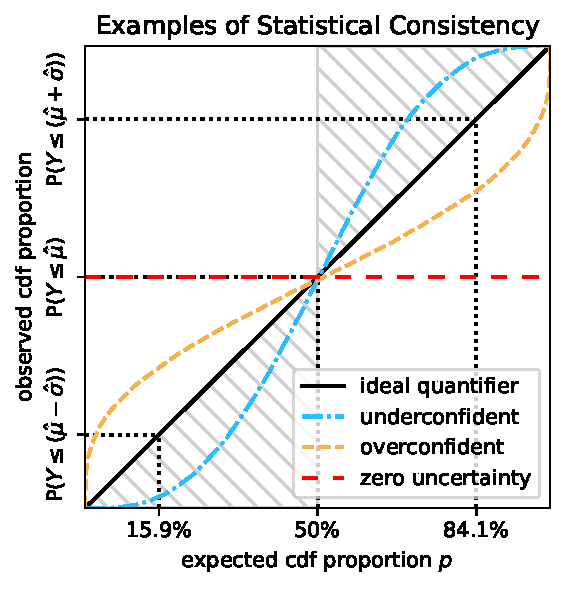
\includegraphics[width=0.325\textwidth]{uncertainty/figures/uq.consistency-examples.pdf}
    \vspace{-1em}
    \caption[Examples of Statistical Consistency Profiles for Uncertainty Quantifiers]{Examples of Statistical Consistency Profiles for Uncertainty Quantifiers}
    \label{fig:uncertainty-consistency}
\end{wrapfigure}

\Cref{fig:uncertainty-consistency} provides several examples of what the calibration plots for different kinds of quantifiers can look like. Note that we only look at uncertainty quantifiers for unbiased predictors here, i.e. models whose prediction is below the true value $50\%$ of the time and above the true value $50\%$ of the time. A quantifier that always predicts zero uncertainty thus produces the red long-dashed horizontal line at $P(Y \leq \hat{\mu}) = 50\%$. Note that a biased predictor shifts the curve upwards if it overestimates the true values but downwards if it underestimates them. Always predicting zero uncertainty is the extreme case of overconfidence, i.e. where the predicted uncertainty is too low. In this case, the predicted confidence intervals are too thin, and the amount of true values below and above the confidence interval is larger than expected. The yellow short-dashed calibration line, which goes through the non-shaded areas of the figure, is an example of such an overconfident quantifier. As its overconfidence grows, its calibration line gets closer to the red long-dashed horizontal line. In contrast, an underconfident quantifier predicts excessive uncertainty, resulting in confidence intervals that are too wide. In this case, the amount of true values below and above the confidence interval is lower than expected, as can be seen with the dash-dotted blue line that stays within the grey-shaded areas. The calibration lines of more underconfident quantifiers approach a vertical line around $p = 50\%$. Finally, an ideal uncertainty quantifier that captures the standard deviation of the error distribution produces the diagonal solid black line in \Cref{fig:uncertainty-consistency}. In our experiments, we also apply both the CRUDE \cite{not-crude-uncertainty-2020, uncertainty-metrics-2023} and CDF-based \cite{uncertainty-calibration-2018, uncertainty-metrics-2023} uncertainty calibration methods with data from a validation dataset to each quantifier. For each of these methods, we show their consistency line and their root-mean-squared-calibration error $RMSCE = \sqrt{\text{E}_{p}[(p - \hat{p})^2]}$ where $\hat{p}$ is the observed cdf proportion. Uncertainty quantifiers with a lower RMSCE are preferred.

While an uncertainty quantifier's RMSCE is usually sufficient to choose the best-performing one, we also investigate two secondary metrics that can serve as tie-breakers, the sharpness and dispersion of the prediction uncertainties, as suggested by \textcite{uncertainty-metrics-2023}. The sharpness metric, as introduced by \textcite{uncertainty-sharpness-2007}, measures the average \textbf{P}rediction \textbf{I}nterval \textbf{W}widths using $PIW = \text{E}[\hat{\sigma}]$. If two quantifiers have similarly high statistical consistency, the one with tighter prediction intervals, i.e. higher sharpness, is preferred. It is crucial to use this secondary metric only for quantifiers with high statistical consistency and not optimise by sharpness alone since that would favour the most overconfident quantifier that always predicts zero uncertainty. In addition to the sharpness, we also calculate dispersion as the predicted \textbf{S}tandard \textbf{D}eviation's \textbf{C}oefficient of \textbf{V}ariation, $SDCV = \sqrt{\text{Var}[\hat{\sigma}]} \mathbin{/} \text{E}[\hat{\sigma}]$, which was introduced by \textcite{uncertainty-dispersion-2019}. This metric rewards quantifiers that further spread out their uncertainty predictions since they may be more robust on unseen data \cite{uncertainty-metrics-2023}. Overall, quantifiers with low $RMSCE$, low $PIW$, and high $SDCV$ are thus preferred. The sharpness and dispersion are shown in the third panel of each figure alongside boxplots that present the median, the $25\%$ and $75\%$ quartiles, and the $5\%$ and $95\%$ range of the uncertainties for the $50\%$-wide and $95\%$-wide confidence intervals for the raw and calibrated quantifiers.

\newpar How would an ideal uncertainty quantifier perform? First, it is worth remembering that an uncertainty quantifier can be ideal even when its prediction model is not. In fact, a quantifier that perfectly predicts the prediction errors or is only evaluated on a predictor without errors should be cause for suspicion. Prediction models and uncertainty quantifiers are generally not perfect. Therefore, an ideal uncertainty quantifier only needs to correctly quantify the uncertainty \textit{distribution} from which the prediction errors are sampled.

\begin{figure}[H]
    \begin{subfigure}
    \centering
    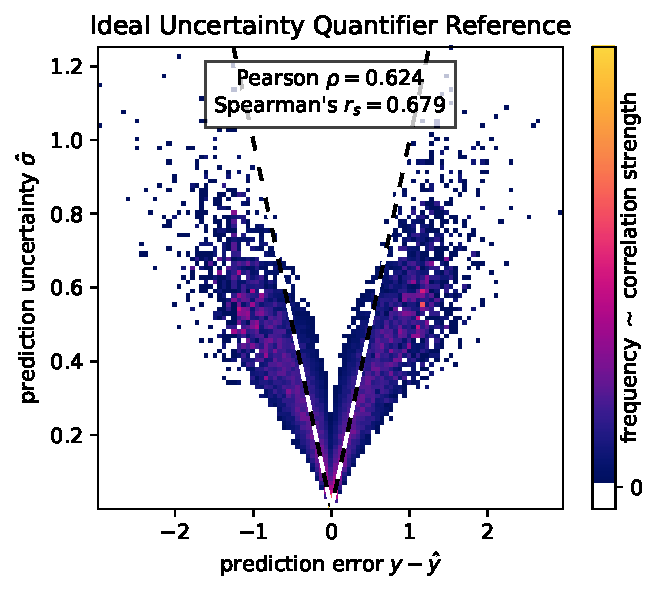
\includegraphics[width=0.348\textwidth,valign=t]{uncertainty/figures/uq.optimaluncertaintyquantifiermodel-correlation.pdf}
    \end{subfigure}
    \begin{subfigure}
    \centering
    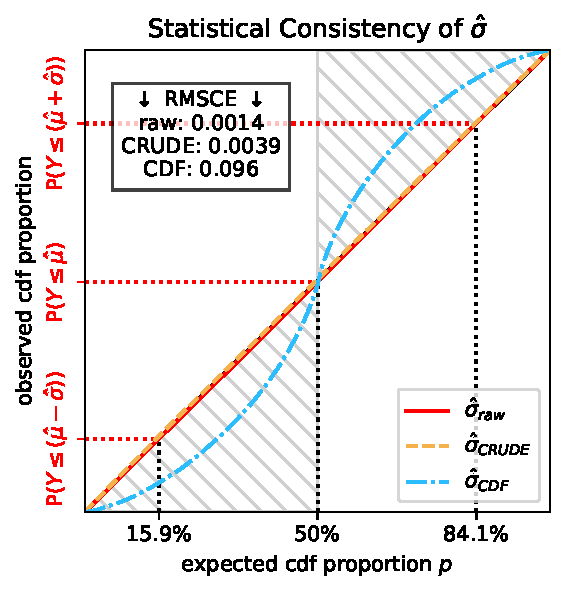
\includegraphics[width=0.299\textwidth,valign=t]{uncertainty/figures/uq.optimaluncertaintyquantifiermodel-consistency.pdf}
    \end{subfigure}
    \begin{subfigure}
    \centering
    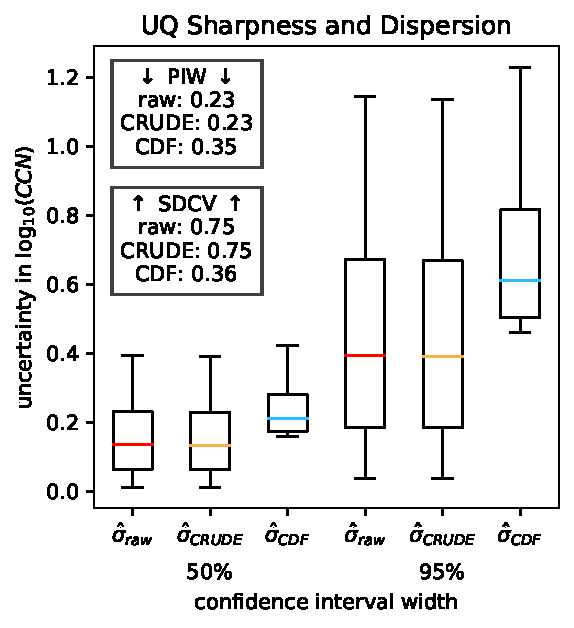
\includegraphics[width=0.303\textwidth,valign=t]{uncertainty/figures/uq.optimaluncertaintyquantifiermodel-sharpness.pdf}
    \end{subfigure}
   
    \vspace{-1em}

    \caption[Reference Example of an ideal Uncertainty Quantifier]{Evaluation of how an ideal Uncertainty Quantifier might perform (see \Cref{txt:uncertainty-methods}) at correlating prediction errors and uncertainties (left), statistical consistency (middle), sharpness and dispersion (right).}
    \label{fig:uncertainty-ideal}
\end{figure}

\noindent We emulate such an ideal uncertainty quantifier by using an oracle to obtain the correct predictions and then adding zero-mean normally-distributed prediction errors with varying standard deviations. We then report these controlled standard deviations as the prediction uncertainties. In the first panel of \Cref{fig:uncertainty-ideal}, we see that even an ideal uncertainty quantifier does not perfectly correlate prediction errors and uncertainties since the former is a random sample and the latter a distribution parameter. The second panel shows that an ideal quantifier has (almost) perfect statistical consistency. It is worth noting that the CDF-based calibration method seems to struggle with this case and predicts underconfident uncertainties. Last but not least, the reasonably low prediction interval width and high dispersion values of the ideal quantifier should only be compared to other quantifiers with error-uncertainty correlation and statistical consistency.

\section{Directly Predicting the Uncertainty Level} \label{txt:uncertainty-predict-sigma}

We first examine the Variance Attenuation method (see \Cref{txt:variance-attenuation}), in which a model is trained to make predictions for both the target value and uncertainty. We follow the recommendation from \textcite{reliable-variance-2019} to train these two submodels separately instead of jointly. Specifically, after a simple predictor $32 \times 32 \times 32$ multi-layer perceptron (MLP) model is optimised with the mean-squared error (MSE) loss, we measure the prediction errors on a disjoint validation set and then train a similar MLP model to predict the uncertainty. This second submodel is trained with the $\beta$-NLL loss (see \Cref{eq:beta-nll-loss}) using $\beta = 0.5$ \cite{beta-nll-2022}.

\begin{figure}[H]
    \begin{subfigure}
    \centering
    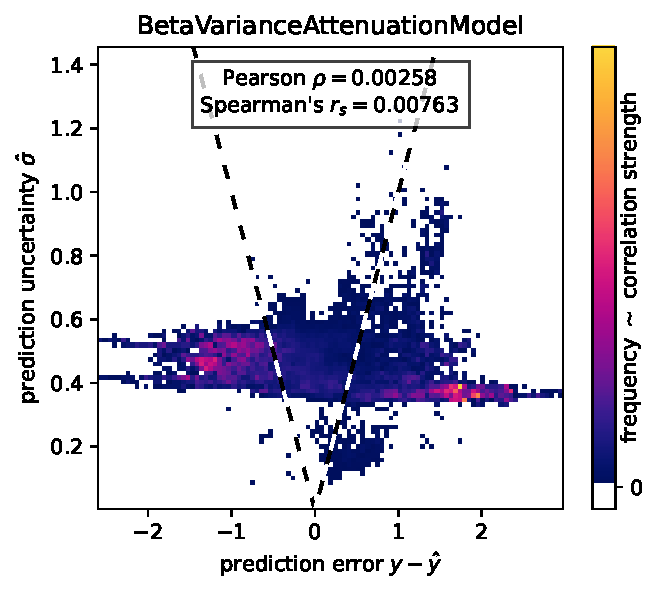
\includegraphics[width=0.345\textwidth,valign=t]{uncertainty/figures/uq.betavarianceattenuationmodel-correlation.pdf}
    \end{subfigure}
    \begin{subfigure}
    \centering
    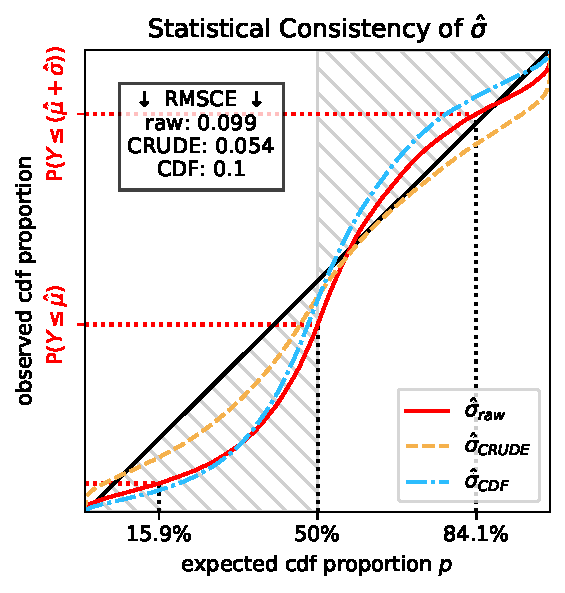
\includegraphics[width=0.297\textwidth,valign=t]{uncertainty/figures/uq.betavarianceattenuationmodel-consistency.pdf}
    \end{subfigure}
    \begin{subfigure}
    \centering
    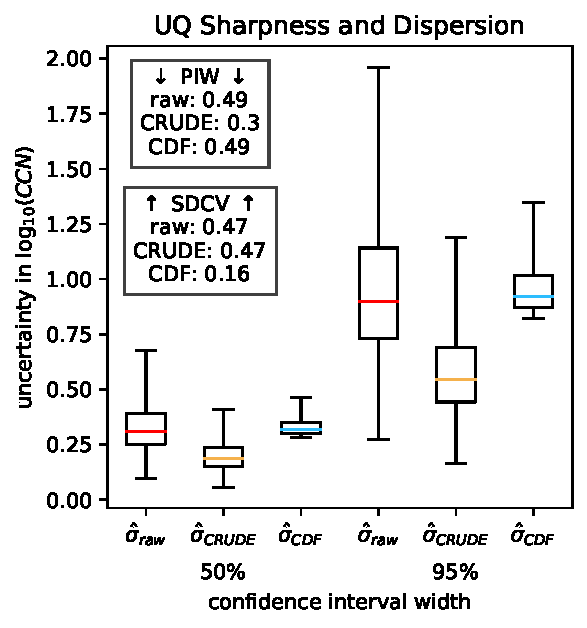
\includegraphics[width=0.308\textwidth,valign=t]{uncertainty/figures/uq.betavarianceattenuationmodel-sharpness.pdf}
    \end{subfigure}
   
    \vspace{-1em}
    \caption[Evaluation of Variance Attenuation as an Uncertainty Quantifier]{Evaluation of Variance Attenuation (see \Cref{txt:variance-attenuation}) as an Uncertainty Quantifier (see \Cref{txt:uncertainty-methods}) based on the correlation between prediction error and uncertainty (left) and the quantifier's statistical consistency (middle), sharpness and dispersion (right).}
    \label{fig:uncertainty-beta-nll}
\end{figure}

\noindent \Cref{fig:uncertainty-beta-nll} shows that this method produces mostly almost-constant uncertainty predictions that are mostly not correlated to the prediction error. Despite the missing correlation, the predicted underconfident level of uncertainty is still somewhat statistically consistent and can be calibrated well using the CRUDE method to have tight prediction intervals with high sharpness and dispersion. In contrast, the CDF-based method results in less consistent and even more underconfident uncertainty predictions. Overall, while Variance Attenuation produces moderately statistically consistent uncertainties, they are heavy-tailed and give no meaningful information about the potential magnitude of the prediction error on the SOSAA data.

\newpar Next, we examine a simpler method for directly predicting the parameters of a normal error distribution. Specifically, we jointly train a combined predictor and quantifier by optimising the predicted normal distribution's negative log-likelihood. The first row in \Cref{fig:uncertainty-normal-gp} shows that this quantifier fares better and produces uncertainty estimates that are lightly correlated to the prediction errors. In addition, the CDF-based calibration is able to improve the statistical consistency and sharpen the prediction intervals at the cost of lower dispersion.

\begin{figure}[H]
    \begin{subfigure}
    \centering
    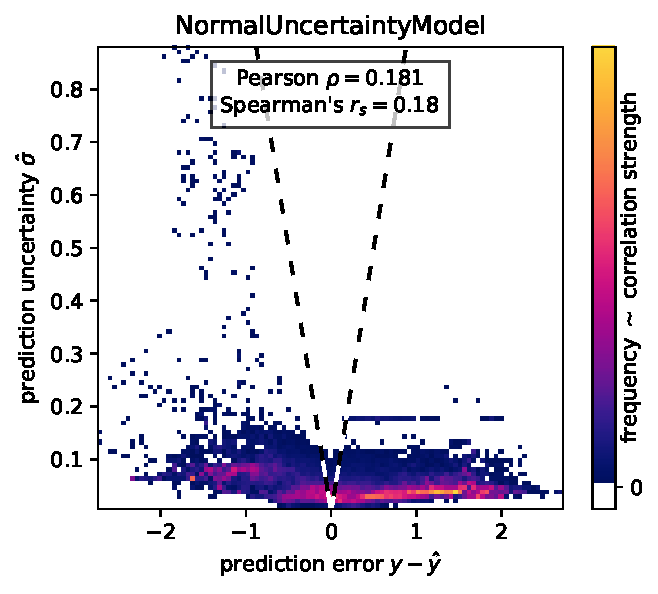
\includegraphics[width=0.345\textwidth,valign=t]{uncertainty/figures/uq.normaluncertaintymodel-correlation.pdf}
    \end{subfigure}
    \begin{subfigure}
    \centering
    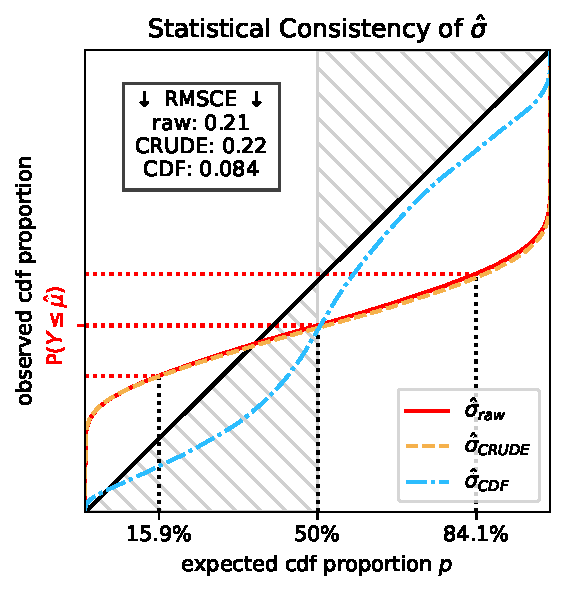
\includegraphics[width=0.297\textwidth,valign=t]{uncertainty/figures/uq.normaluncertaintymodel-consistency.pdf}
    \end{subfigure}
    \begin{subfigure}
    \centering
    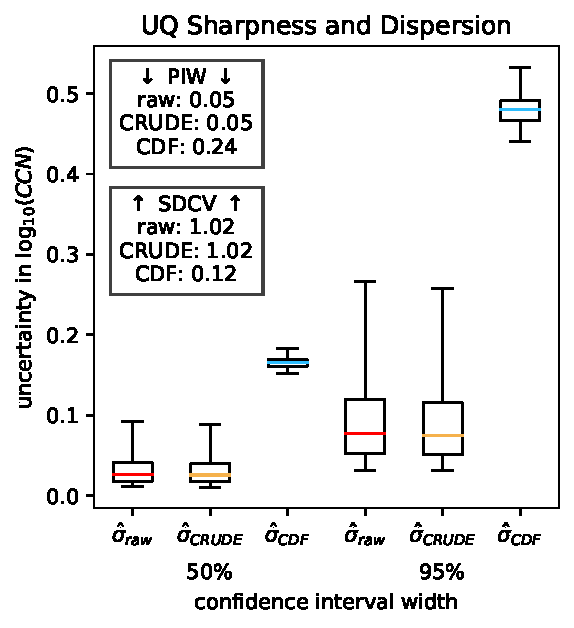
\includegraphics[width=0.308\textwidth,valign=t]{uncertainty/figures/uq.normaluncertaintymodel-sharpness.pdf}
    \end{subfigure}

    \begin{subfigure}
    \centering
    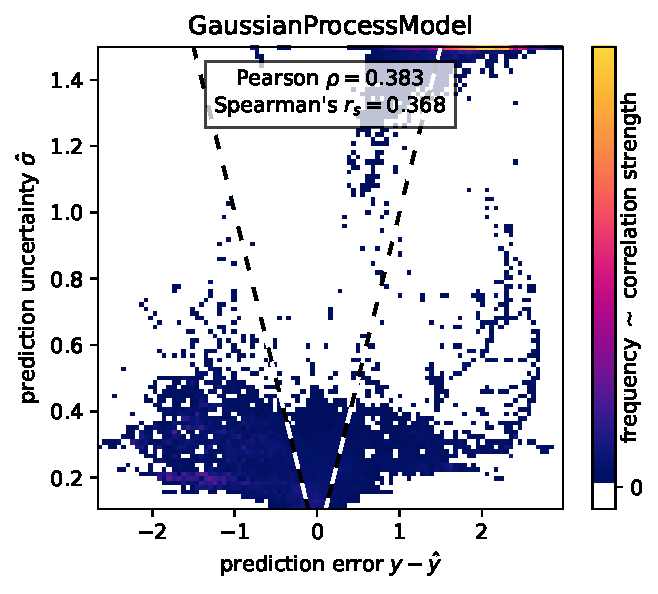
\includegraphics[width=0.345\textwidth,valign=t]{uncertainty/figures/uq.gaussianprocessmodel-correlation.pdf}
    \end{subfigure}
    \begin{subfigure}
    \centering
    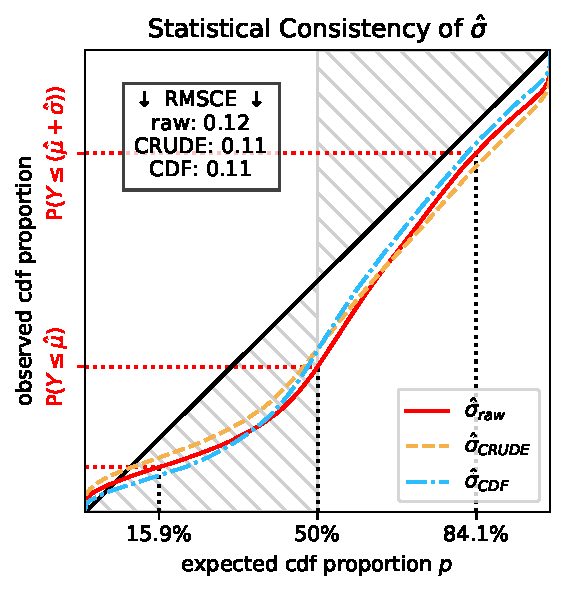
\includegraphics[width=0.297\textwidth,valign=t]{uncertainty/figures/uq.gaussianprocessmodel-consistency.pdf}
    \end{subfigure}
    \begin{subfigure}
    \centering
    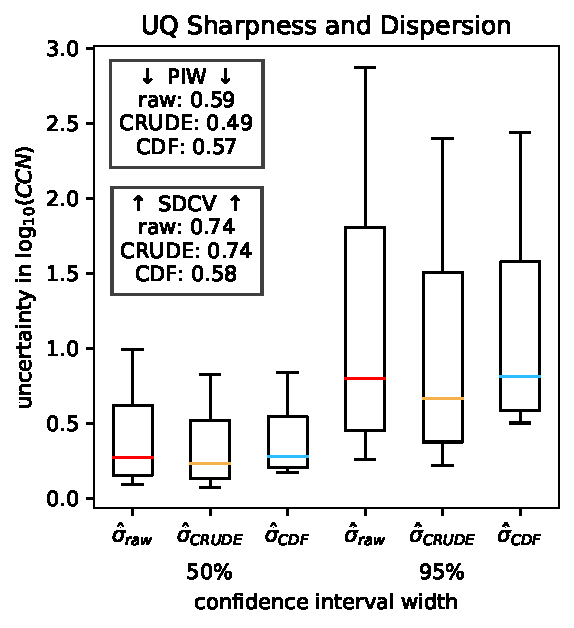
\includegraphics[width=0.308\textwidth,valign=t]{uncertainty/figures/uq.gaussianprocessmodel-sharpness.pdf}
    \end{subfigure}
   
    \vspace{-1em}
    \caption[Evaluation of Normal Errors and Gaussian Processes as Uncertainty Quantifiers]{Evaluation of Normal-distributed Errors and Gaussian Processes (see \Cref{txt:gaussian-process}) as Uncertainty Quantifiers (see \Cref{txt:uncertainty-methods}) based on the correlation between prediction error and uncertainty (left) and the quantifier's statistical consistency (middle), sharpness and dispersion (right).}
    \label{fig:uncertainty-normal-gp}
\end{figure}

\noindent We also again test Gaussian Processes (GPs), whose predictive performance was already analysed in \Cref{fig:bayesian-gp-models}. We again subsample the combined training data of all trajectories to make the training computationally feasible. While GPs achieve the second-highest correlation score, the correlation plot in \Cref{fig:uncertainty-normal-gp} shows a clear asymmetry between positive and negative prediction errors, signalling instability. Furthermore, the GP consistently makes underpredictions on the test data. Unfortunately, calibration is unable to improve upon this inconsistency. Thus, GPs are not well-suited to quantify uncertainty on the SOSAA trajectories dataset.

\section{Estimating a Model's Prediction Errors} \label{txt:uncertainty-predict-error}

Another intuitive approach for uncertainty quantification is to train a second model that predicts the prediction errors $y - \hat{y}$ that the first makes, i.e. its residuals. In our first experiment, we use a simple $32 \times 32 \times 32$ MLP to estimate the prediction error of a similar network. The first row in \Cref{fig:uncertainty-residual-rio} shows that this method is unable to capture the correlation between prediction errors and uncertainty. While both validation-data-based calibration methods succeed in turning the overconfident uncertainty predictions into preferable underconfident ones, they overestimate the correction needed.

\begin{figure}[H]
    \begin{subfigure}
    \centering
    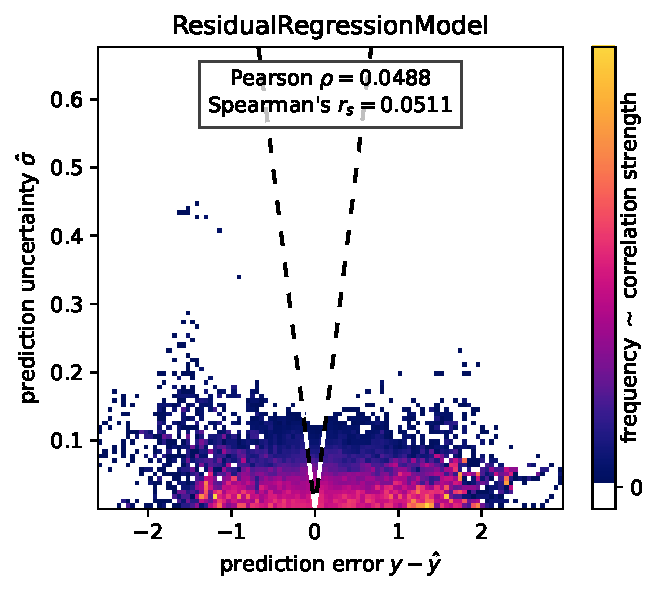
\includegraphics[width=0.349\textwidth,valign=t]{uncertainty/figures/uq.residualregressionmodel-correlation.pdf}
    \end{subfigure}
    \begin{subfigure}
    \centering
    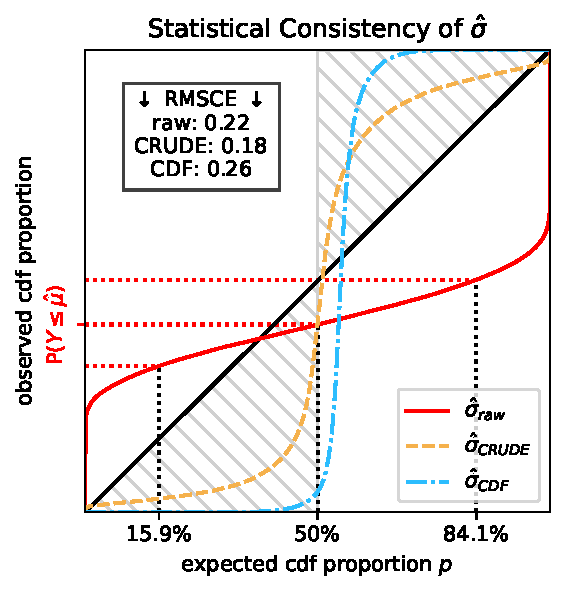
\includegraphics[width=0.300\textwidth,valign=t]{uncertainty/figures/uq.residualregressionmodel-consistency.pdf}
    \end{subfigure}
    \begin{subfigure}
    \centering
    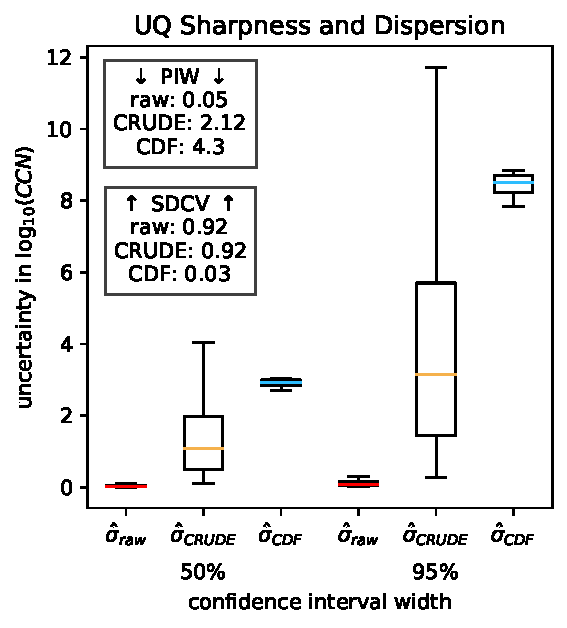
\includegraphics[width=0.301\textwidth,valign=t]{uncertainty/figures/uq.residualregressionmodel-sharpness.pdf}
    \end{subfigure}
   
    \begin{subfigure}
    \centering
    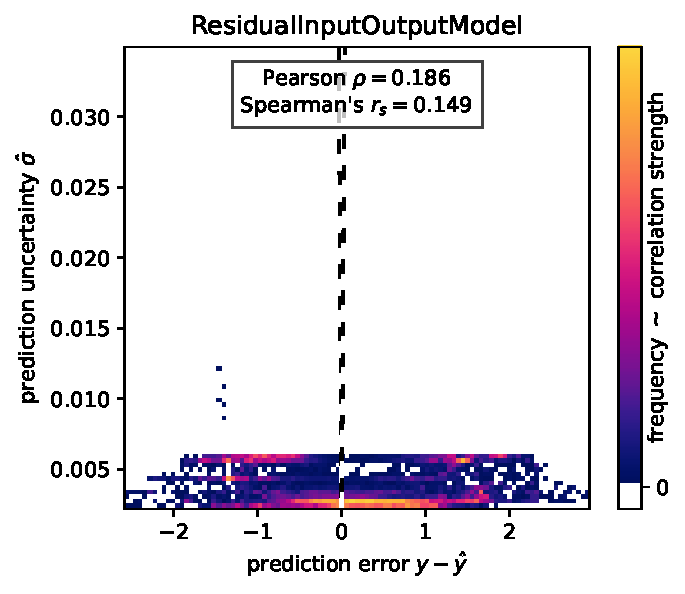
\includegraphics[width=0.358\textwidth,valign=t]{uncertainty/figures/uq.residualinputoutputmodel-correlation.pdf}
    \end{subfigure}
    \begin{subfigure}
    \centering
    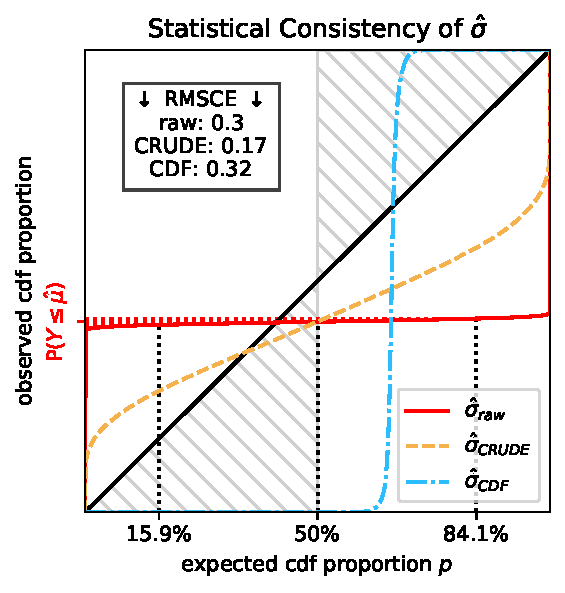
\includegraphics[width=0.295\textwidth,valign=t]{uncertainty/figures/uq.residualinputoutputmodel-consistency.pdf}
    \end{subfigure}
    \begin{subfigure}
    \centering
    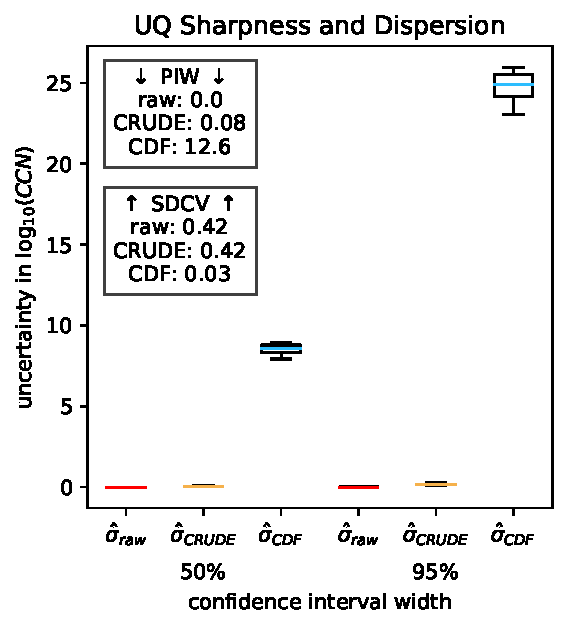
\includegraphics[width=0.297\textwidth,valign=t]{uncertainty/figures/uq.residualinputoutputmodel-sharpness.pdf}
    \end{subfigure}

    \vspace{-1em}
    \caption[Evaluation of Uncertainty Quantifiers based on Residual Regression]{Evaluation of Residual Regression using a Neural Network or Gaussian Process \cite{rio-2019} as Uncertainty Quantifiers (see \Cref{txt:uncertainty-methods}) based on the correlation between prediction error and uncertainty (left) and the quantifier's statistical consistency (middle), sharpness and dispersion (right).}
    \label{fig:uncertainty-residual-rio}
\end{figure}

\noindent \textcite{rio-2019} present the RIO method, which uses Gaussian Processes to estimate the covariance of the zero-mean normally-distributed prediction residuals of an existing predictor model and calibrate its prediction. Specifically, the authors propose training the GP with a combined input-output (IO) kernel, which consists of one radial basis function kernel for the inputs $X$ and one for the base model predictions $\hat{Y}$. The mean residual prediction from this GP is added to $\hat{Y}$ to improve the base model's prediction. While RIO improves the correlation between prediction errors and uncertainties, the second row of \Cref{fig:uncertainty-residual-rio} also shows that the method massively underestimates the prediction uncertainty. While the CRUDE calibration method is able to make the quantifier less overconfident, the CDF-based method again highly overshoots. In particular, for a prediction range of roughly $10^{4} \leq CCN \leq 10^{11}$, it predicts $95\%$-wide confidence intervals with widths of $10^{25}$. However, if we stick with the CRUDE calibration method, RIO does present an improvement by decreasing both the $RMSCE$ and $PIW$ over the MLP-based residual regression uncertainty quantifier.

\section{Predicting Prediction Ranges} \label{txt:uncertainty-predict-range}

Estimating the range of values the target value is most likely in is an approach for uncertainty quantification. For instance, Quantile Regression trains one or more submodels to predict one quantile $q \in [0; 1]$ of the target function each, in our case the median at $50\%$ and the $\pm \sigma$ quantiles at approximately $15.9\%$ and $84.1\%$. Note that, unlike the previous methods, the estimated uncertainty range can now be asymmetric around the prediction mean. Each quantile submodule is optimised to predict $\hat{y}_{q}$ with the following pinball loss function \cite{regression-quantiles-1978, deep-quantiles-2022}:
\begin{equation*}
    \mathcal{L} = \begin{cases}
        q \cdot \mathcal{L}_{raw} \quad &\text{if } \mathcal{L}_{raw} \geq 0 \\
        (1-q) \cdot \mathcal{L}_{raw} \quad &\text{otherwise}
    \end{cases} \quad \text{where} \quad \mathcal{L}_{raw} = y - \hat{y}_{q}
\end{equation*}
We then estimate the prediction uncertainty as $\hat{\sigma} = 0.5 \cdot |\hat{y}_{84.1\%} - \hat{y}_{15.9\%}|$. The first row in \Cref{fig:uncertainty-quantile-interval} shows that this method produces lightly correlated uncertainty estimates, which are only beaten by Random Forests (see \Cref{fig:uncertainty-rf-mc-dropout}) and Gaussian Processes, the latter of which suffers from asymmetry (see \Cref{fig:uncertainty-normal-gp}). Unfortunately, the calibration of the underestimations with overconfident uncertainty predictions is yet again unsuccessful as both calibration methods overshoot into high underconfidence.

\begin{figure}[H]
    \begin{subfigure}
    \centering
    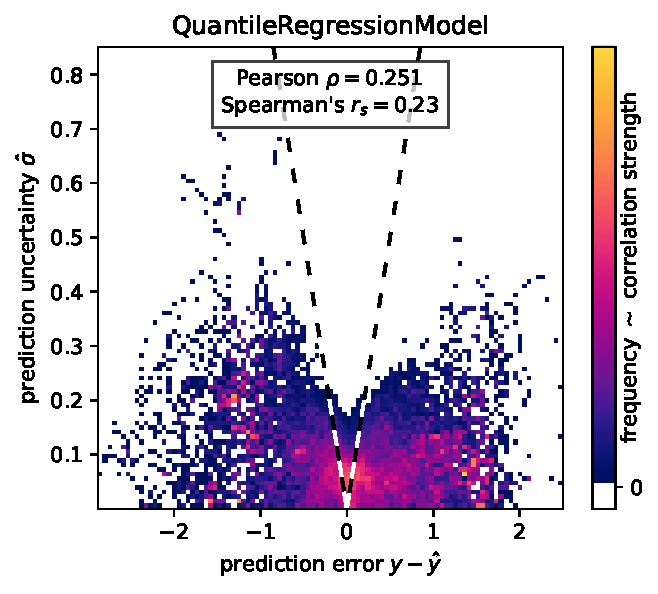
\includegraphics[width=0.345\textwidth,valign=t]{uncertainty/figures/uq.quantileregressionmodel-correlation.pdf}
    \end{subfigure}
    \begin{subfigure}
    \centering
    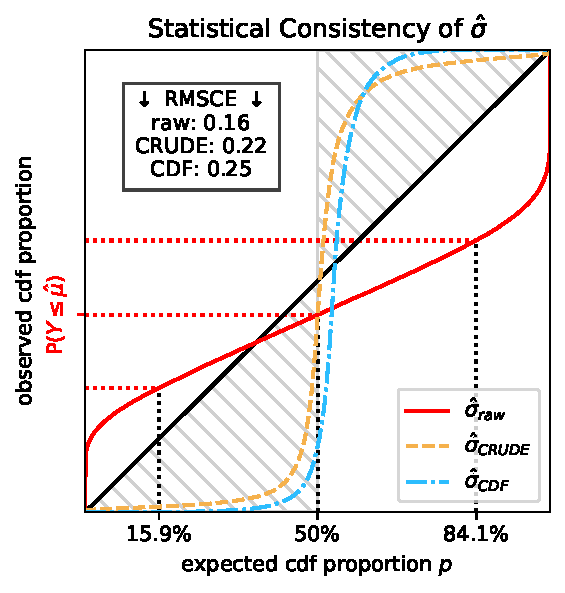
\includegraphics[width=0.297\textwidth,valign=t]{uncertainty/figures/uq.quantileregressionmodel-consistency.pdf}
    \end{subfigure}
    \begin{subfigure}
    \centering
    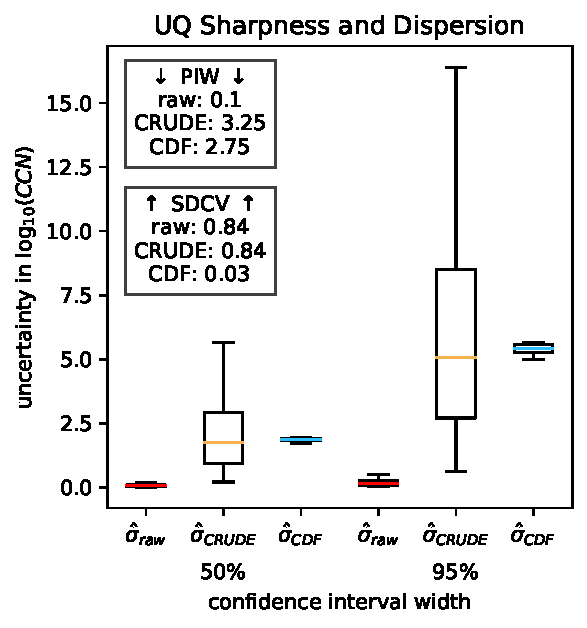
\includegraphics[width=0.308\textwidth,valign=t]{uncertainty/figures/uq.quantileregressionmodel-sharpness.pdf}
    \end{subfigure}

    \begin{subfigure}
    \centering
    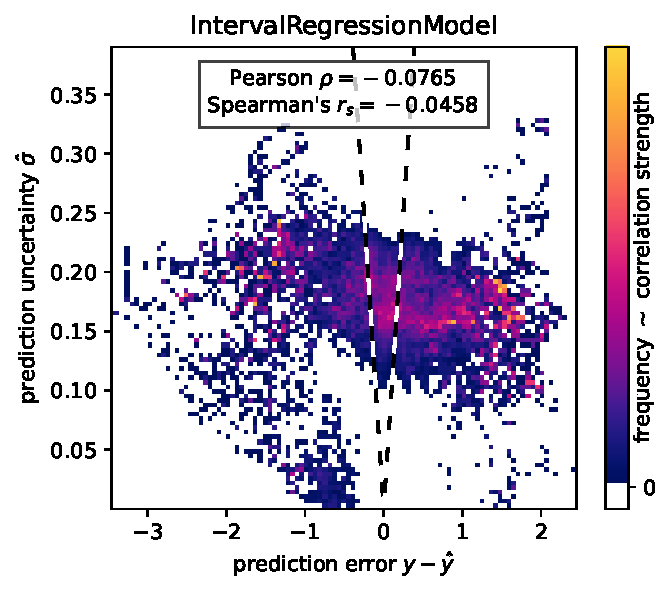
\includegraphics[width=0.351\textwidth,valign=t]{uncertainty/figures/uq.intervalregressionmodel-correlation.pdf}
    \end{subfigure}
    \begin{subfigure}
    \centering
    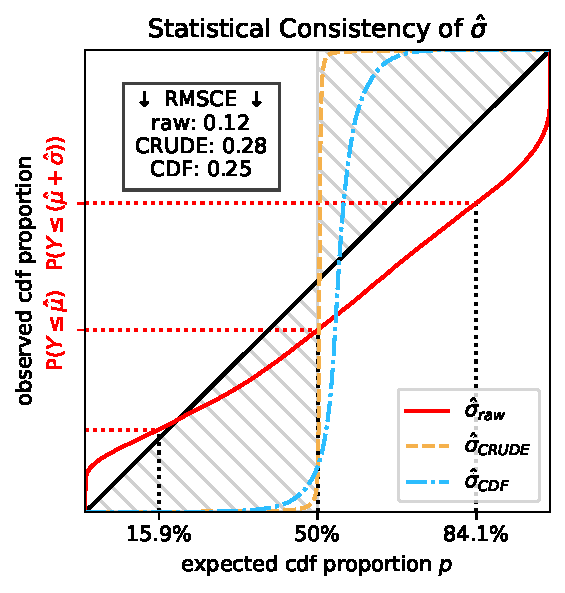
\includegraphics[width=0.296\textwidth,valign=t]{uncertainty/figures/uq.intervalregressionmodel-consistency.pdf}
    \end{subfigure}
    \begin{subfigure}
    \centering
    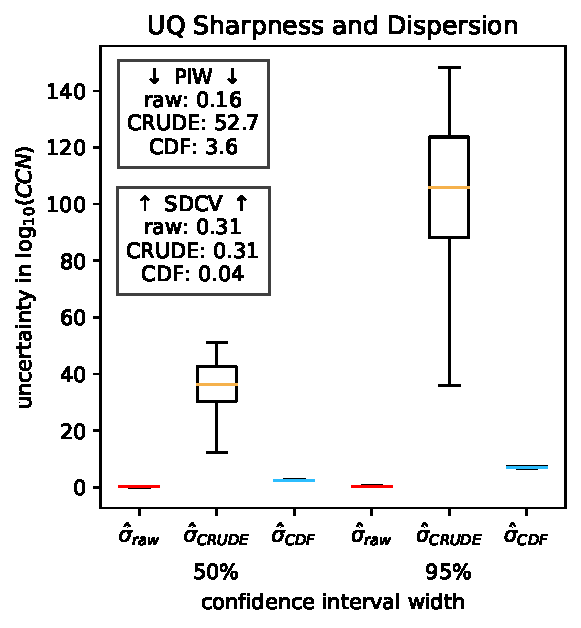
\includegraphics[width=0.303\textwidth,valign=t]{uncertainty/figures/uq.intervalregressionmodel-sharpness.pdf}
    \end{subfigure}
   
    \vspace{-1em}
    \caption[Evaluation of Quantile and Interval Regression as Uncertainty Quantifiers]{Evaluation of Quantile Regression \cite{regression-quantiles-1978, deep-quantiles-2022} and Interval Regression \cite{interval-minimisation-2018} as Uncertainty Quantifiers (see \Cref{txt:uncertainty-methods}) based on the correlation between prediction error and uncertainty (left) and the quantifier's statistical consistency (middle), sharpness and dispersion (right).}
    \label{fig:uncertainty-quantile-interval}
\end{figure}

\noindent Expanded Interval Minimization is a similar approach by \textcite{interval-minimisation-2018} that aims to estimate the lower and upper bound of the as-tight-as-possible prediction interval that contains the true target with some configurable probability. In addition to predicting the bounds, the interval width predictions are rescaled across each training batch such that the expected percentage of true values falls within them. After training, a similar final calibration is performed on a validation data set. In this experiment, we again use the $15.9\%$ and $84.1\%$ quantiles to learn the prediction interval that should cover the $\mu \pm \sigma$ range. The second row in \Cref{fig:uncertainty-quantile-interval} shows that this method is, unfortunately, unable to produce error-correlated uncertainty estimates. Furthermore, both calibration methods fail to correct the underestimation bias on the test data. This example also showcases an example where the CRUDE calibration fails, resulting in excessively high underconfidence.

\section{The Success of Ensemble Methods} \label{txt:uncertainty-ensemble-methods}

Ensemble methods combine the predictions from several models (see \Cref{txt:ensembles-decision-tree-random-forest}), which can both improve the quality of the overall prediction and be used to measure prediction uncertainty as the variation amongst ensemble predictions. The first row of \Cref{fig:uncertainty-rf-mc-dropout} evaluates the performance of Random Forests (RFs), which consist of an ensemble of decision tree regressors, here ten. The left plot shows that this method's prediction uncertainty correlates well with the RF's mean prediction error. In fact, Random Forests have the highest correlation scores among our experiments and get close to the optimal uncertainty quantifier's correlation score (see \Cref{fig:uncertainty-ideal}). Furthermore, it is the only method whose Spearman's rank correlation coefficient is significantly larger than its Pearson correlation, which is also observed for the ideal quantifier. The uncalibrated RF predictions have high statistical consistency but are slightly overconfident. The RF also produces sharp prediction intervals, which are only tighter for the Normal error distribution method (see \Cref{fig:uncertainty-normal-gp}). Unfortunately, calibration is unable to improve the already high statistical consistency of the RF uncertainty further: CRUDE results in even higher overconfidence, while the CDF-based method overshoots into underconfident uncertainty predictions.

\begin{figure}[H]
    \begin{subfigure}
    \centering
    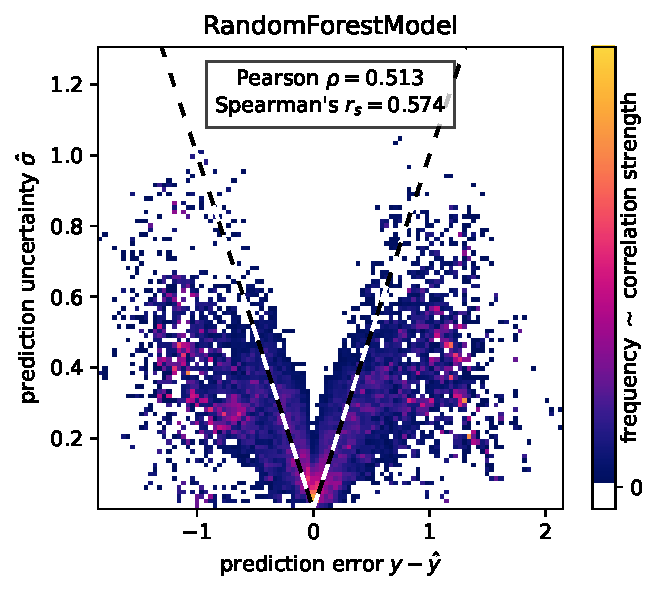
\includegraphics[width=0.348\textwidth,valign=t]{uncertainty/figures/uq.randomforestmodel-correlation.pdf}
    \end{subfigure}
    \begin{subfigure}
    \centering
    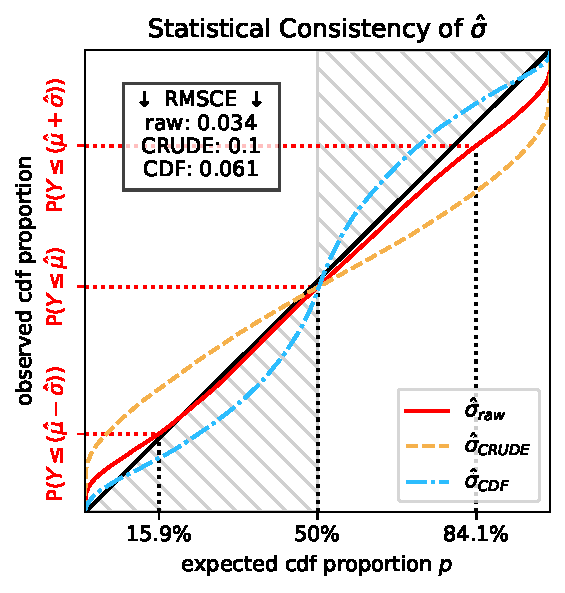
\includegraphics[width=0.299\textwidth,valign=t]{uncertainty/figures/uq.randomforestmodel-consistency.pdf}
    \end{subfigure}
    \begin{subfigure}
    \centering
    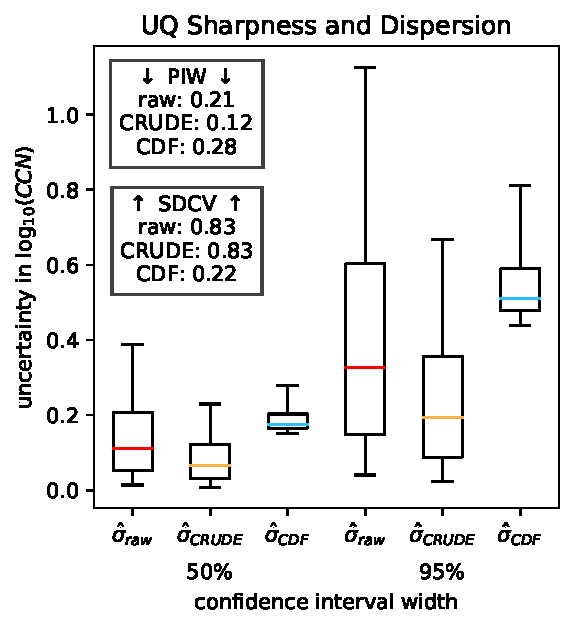
\includegraphics[width=0.303\textwidth,valign=t]{uncertainty/figures/uq.randomforestmodel-sharpness.pdf}
    \end{subfigure}

    \begin{subfigure}
    \centering
    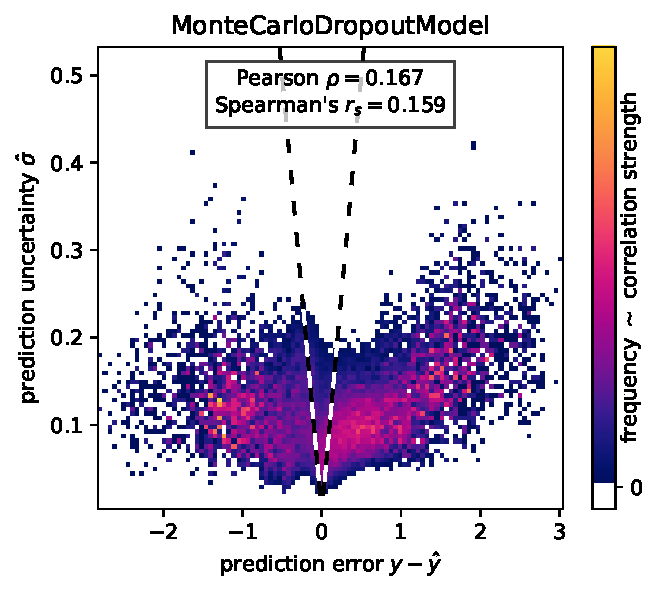
\includegraphics[width=0.348\textwidth,valign=t]{uncertainty/figures/uq.montecarlodropoutmodel-correlation.pdf}
    \end{subfigure}
    \begin{subfigure}
    \centering
    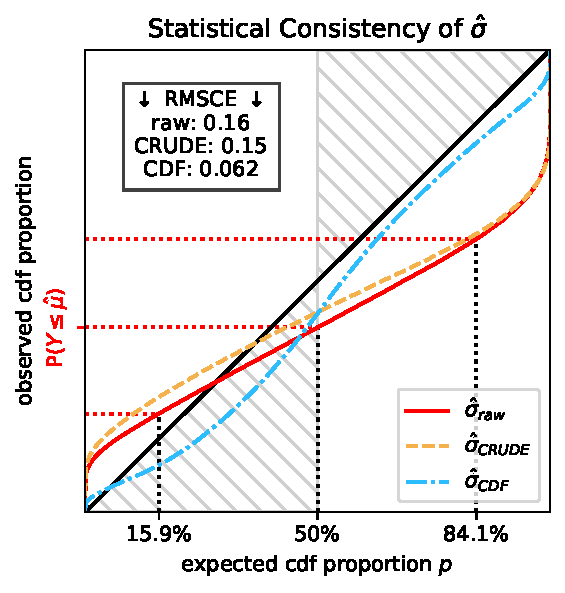
\includegraphics[width=0.299\textwidth,valign=t]{uncertainty/figures/uq.montecarlodropoutmodel-consistency.pdf}
    \end{subfigure}
    \begin{subfigure}
    \centering
    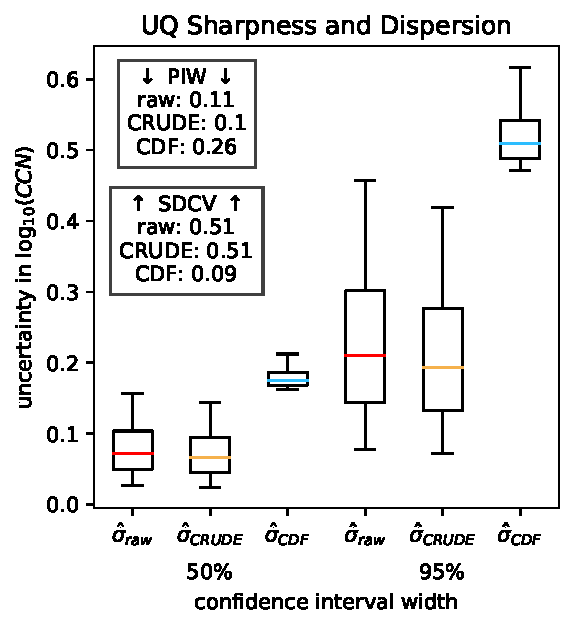
\includegraphics[width=0.303\textwidth,valign=t]{uncertainty/figures/uq.montecarlodropoutmodel-sharpness.pdf}
    \end{subfigure}
   
    \vspace{-1em}
    \caption[Evaluation of Random Forests and Monte Carlo Dropout as Uncertainty Quantifiers]{Evaluation of Random Forests (see \Cref{txt:ensembles-decision-tree-random-forest}) and Monte Carlo Dropout (see \Cref{txt:mc-dropout}) as Uncertainty Quantifiers (see \Cref{txt:uncertainty-methods}) based on the correlation between prediction error and uncertainty (left) and the quantifier's statistical consistency (middle), sharpness and dispersion (right).}
    \label{fig:uncertainty-rf-mc-dropout}
\end{figure}

\noindent Monte Carlo (MC) Dropout builds an ensemble of neural networks without needing to train several submodels. In particular, it uses dropout layers, which randomly replace the previous layer's outputs with zero, during training \textit{and} also during deployment. Thus, when the model is asked several times to make a prediction, it produces an ensemble of several independent predictions. Our experiments use ten samples and a dropout rate of $0.1$ \cite{mc-dropout-2016}. The second row of \Cref{fig:uncertainty-rf-mc-dropout} shows that the obtained uncertainties are only lightly correlated to the prediction errors, less than the Random Forest's. The uncertainty predictions produced by MC dropout are overconfident, which the CDF-based calibration method is able to improve upon. However, this calibration struggles from wider, less sharp and less dispersed uncertainties than the uncalibrated quantifier.

\newpar Finally, we also again investigate Pairwise Difference Regression using Random Forests (PADRE-RF), which is introduced in \Cref{txt:padre-rf}. PADRE-RF is similar to both Random Forests and Monte Carlo Dropout as it is built with an ensemble of decision trees \textit{and} evaluated several times to produce a set of random predictions. As already seen in \Cref{txt:model-evaluation}, PADRE-RF's predictions are very noisy (see \Cref{fig:rf-padre-rf-models}) and have high uncertainty, which the first row in \Cref{fig:uncertainty-padre-residual} reflects. This plot also validates our earlier analysis that the correlation between the prediction error and uncertainty is only weak. Surprisingly, PADRE-RF produces the most statistically consistent uncertainties when calibrated using the CRUDE method, without which it is slightly underconfident.

We also briefly explore whether PADRE-RF as a prediction model can be combined with a Gaussian Process to predict the error residuals and quantify the prediction uncertainty. Specifically, the uncertainty quantifier is based on the RIO method from \Cref{fig:uncertainty-residual-rio}. The second row in \Cref{fig:uncertainty-padre-residual} unfortunately shows that this approach produces uncertainty estimates which are not correlated with the prediction error. Why does this combination still have high statistical consistency? If the prediction errors are drawn from one input-independent normal distribution, the uncertainty quantifier only needs to learn this distribution's constant standard deviation. The correlation plot for the PADRE-RF-RIO combination shows that most uncertainty predictions are indeed inside a tiny band of values between $0.3$ and $0.4$, which supports our explanation. Since the combined method does not change the prediction error range and performs worse than PADRE-RF by itself, we do not explore it further.

\begin{figure}[H]
    \begin{subfigure}
    \centering
    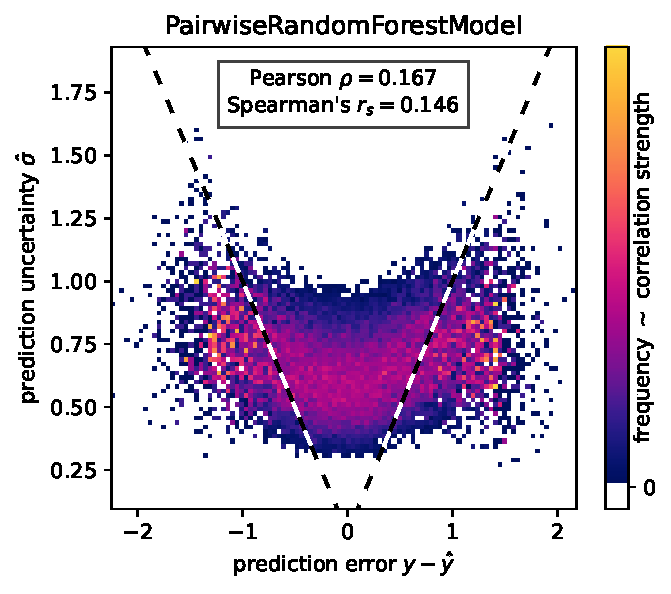
\includegraphics[width=0.350\textwidth,valign=t]{uncertainty/figures/uq.pairwiserandomforestmodel-correlation.pdf}
    \end{subfigure}
    \begin{subfigure}
    \centering
    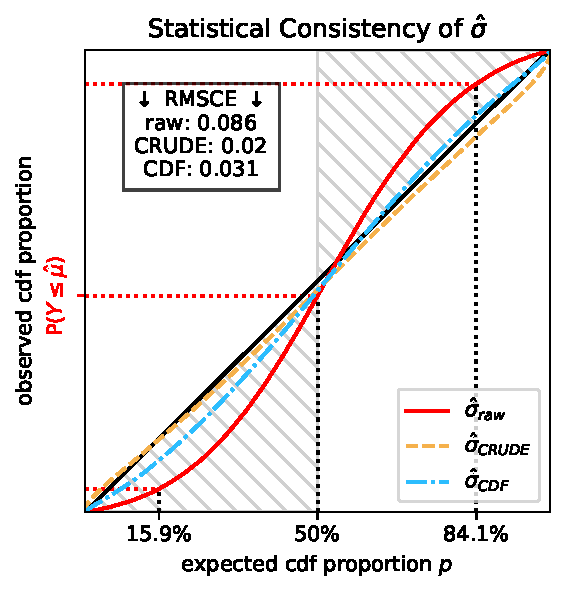
\includegraphics[width=0.295\textwidth,valign=t]{uncertainty/figures/uq.pairwiserandomforestmodel-consistency.pdf}
    \end{subfigure}
    \begin{subfigure}
    \centering
    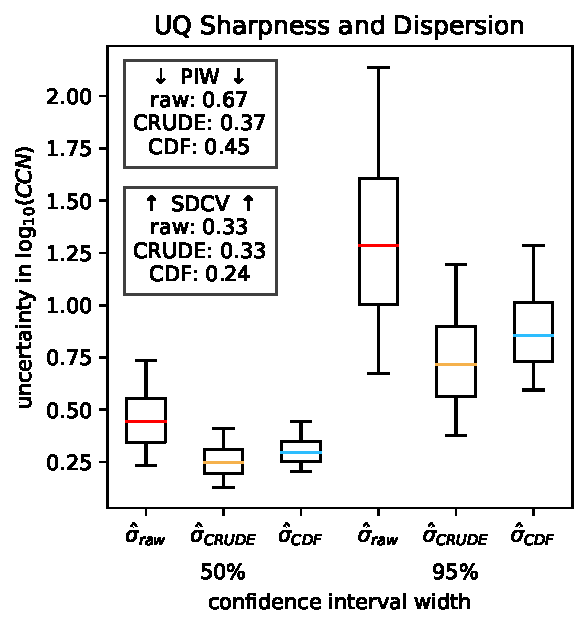
\includegraphics[width=0.305\textwidth,valign=t]{uncertainty/figures/uq.pairwiserandomforestmodel-sharpness.pdf}
    \end{subfigure}

    \begin{subfigure}
    \centering
    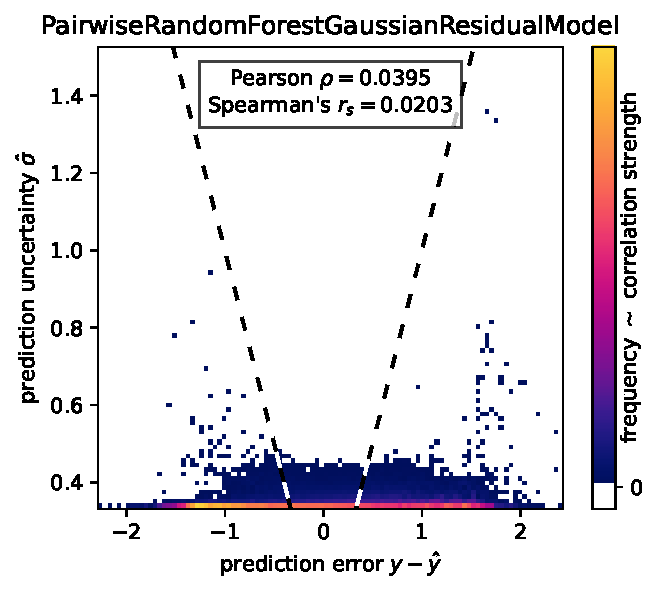
\includegraphics[width=0.348\textwidth,valign=t]{uncertainty/figures/uq.pairwiserandomforestgaussianresidualmodel-correlation.pdf}
    \end{subfigure}
    \begin{subfigure}
    \centering
    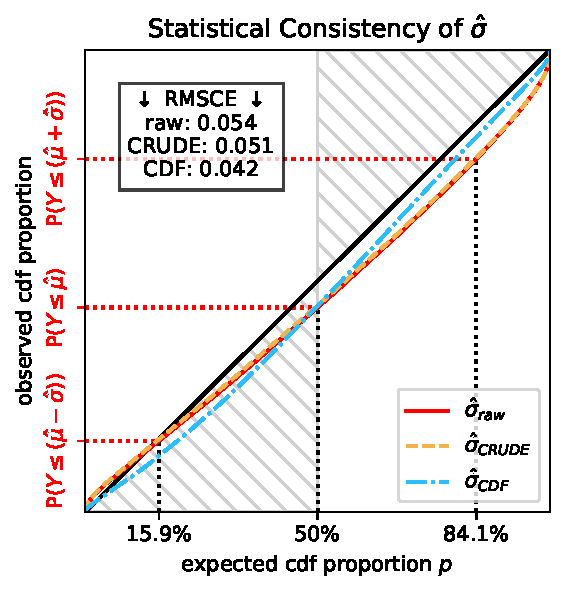
\includegraphics[width=0.299\textwidth,valign=t]{uncertainty/figures/uq.pairwiserandomforestgaussianresidualmodel-consistency.pdf}
    \end{subfigure}
    \begin{subfigure}
    \centering
    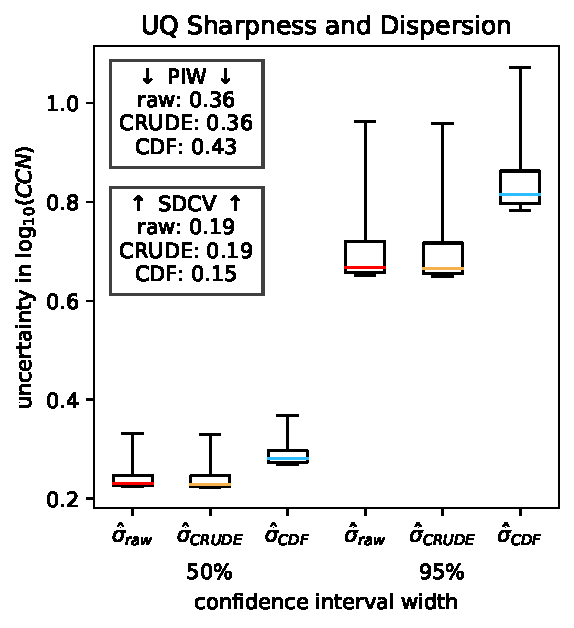
\includegraphics[width=0.303\textwidth,valign=t]{uncertainty/figures/uq.pairwiserandomforestgaussianresidualmodel-sharpness.pdf}
    \end{subfigure}
   
    \vspace{-1em}
    \caption[Evaluation of PADRE-RF as an Uncertainty Quantifier]{Evaluation of Pairwise Difference Regression with Random Forests (see \Cref{txt:padre-rf}), optionally with RIO Residuals, as Uncertainty Quantifiers (see \Cref{txt:uncertainty-methods}) based on the correlation between prediction error and uncertainty (left) and the quantifier's statistical consistency (middle), sharpness and dispersion (right).}
    \label{fig:uncertainty-padre-residual}
\end{figure}

\section{Reflections on Uncertainty Quantification} \label{txt:uncertainty-conclusions}

This chapter has evaluated the performance of several uncertainty quantification methods on the SOSAA trajectories dataset. Our experiments show that methods which directly predict the uncertainty level or attempt to estimate the prediction error struggle. Instead, joint predictor-quantifier ensemble methods should be chosen since they ask what range of models can be learned with some training data and, thus, which range of predictions can be made. In particular, Random Forests stand out with the highest error-uncertainty correlation and most statistically consistent uncertainties if no calibration is used.

It is again important to refer back to \Cref{fig:uncertainty-ideal}, which explored what the performance profile of an ideal uncertainty quantifier might look like. Real-world uncertainty quantifiers do not produce perfect error-uncertainty correlations. Instead, high statistical consistency and strong correlations are the two primary criteria to look for since they allow the predicted uncertainty levels to be interpreted intuitively.

We thus also want to highlight CRUDE-calibrated PADRE-RF, which produces larger uncertainty but is slightly more statistically consistent than RFs. Why are statistically consistent predictions preferable to more accurate but inconsistent predictions in our project? The predictions that the Icarus RSM makes are not the end product but are intended to be used in further downstream analysis. If the prediction uncertainty is correctly predicted, it can be passed through this analysis and be presented to the user as uncertainty bounds on the final analysis result. In contrast, less consistent uncertainty predictions also make the final analysis uncertainty less valuable to base conclusions on. Therefore, PADRE-RF also is a promising candidate for both prediction and uncertainty quantification.

\newpar We have now explored all three parts of the Icarus RSM (see \Cref{txt:icarus-rsm}). Next, \Cref{txt:icarus-evaluation-chapter} builds upon our conclusions from \Cref{txt:ood-detection-chapter}, \Cref{txt:prediction-chapter}, and \Cref{txt:uncertainty-chapter} to construct a baseline SOSAA RSM implementation to implement the combined performance of an OOD detector, a prediction model, and an uncertainty quantifier.
